\documentclass[12pt]{article}
\usepackage[utf8]{inputenc}
\usepackage[legalpaper, portrait, margin=0.8in]{geometry}
\usepackage{amssymb}
\usepackage{amsmath}
\usepackage{graphicx}

\title{CDA5106 - Advanced Computer Architecture \\ Practice Examples}
\author{Kobee Raveendran}
\date{}

\begin{document}
    \maketitle

    \section{Module 1: High-Performance Microprocessor Architecture}

    \subsection{Dennard Scaling}

    \begin{enumerate}
        \item Suppose that instead of progressing at a ratio of 0.7, Moore’s law slows down and transistor gate length scales at a ratio of 0.8 instead. Find the dynamic power consumption under \textit{unlimited} and \textit{limited} scaling for the next process generation.

        \begin{itemize}
            \item Unlimited/old scaling rule
            \begin{itemize}
                \item gate length scales by $S = 0.8$
                \item capacitance scales by $S = 0.8$
                \item original area scales by $S^2 = 0.64$
                \item num transistors thus scales by $\frac{1}{S^2} = 1.56$
                \item supply voltage scales by $S = 0.8$
                \item frequency scales by $\frac{1}{S} = 1.25$
                \item dynamic power stays constant:
            
                $P_{dyn} = (1.56A)(0.8C)(0.8V)^2(1.25f)$
            \end{itemize}
            
            \item leakage-limited/new scaling
            \begin{itemize}
                \item capacitance scales by $S = 0.8$
                \item num transistors scales by $\frac{1}{S^2} = 1.56$
                \item supply voltage does not scale without scaling threshold voltage too, which increases static power exponentially
                \item frequency scales by $\frac{1}{S} 1.25$
                \item dynamic power consumption increases:

                $P_{dyn}' = (1.56A)(0.8C)(V)^2(1.25f) = 1.56 \cdot P_{dyn}$
            \end{itemize}
        \end{itemize}

        \item With limited voltage scaling, suppose that we want to keep the dynamic power consumption constant in the next generation by keeping frequency constant and reduce die area. How much should we reduce die area to achieve that?
        \begin{itemize}
            \item gate length scales by $S = 0.7$
            \item capacitance scales by $S = 0.7$
            \item original area scales by $S^2 = 0.5$
            \item supply voltage and frequency are constant
            \item dynamic power consumption must stay constant: $P_{dyn}' = P_{dyn}$

            $ACV^2f = A'(0.7C)V^2f \longrightarrow A = 0.7A'$

            \item number of transistors in the next generation: $A' = 1.4A$ (instead of 2A like before; i.e. 70\% of 2A)
            \item thus die area shrinks by 30\%
        \end{itemize}

        \item Describe the difference between energy and power.

        Power is the rate of energy consumption.

        \item Describe the impact of threshold voltage choice on static and dynamic power consumption as transistors are scaled down.

        If threshold voltage is lowered, dynamic power decreases (nearly linearly) but static power increases exponentially.

        \item How has processor design adapted to the power wall problem?

        Stalling frequency growth, multicore, and sophisticated power management (clock gating, voltage and frequency scaling, power gating).
    \end{enumerate}

    \section{Module 2: Performance, Cost, and Reliability of Microprocessors}

    \subsection{Amdahl's Law}

    Example:

	\begin{itemize}
		\item jet plane wing simulation, where 1 run takes 1 week on your computer
		\item your program is 80\% parallelizable
		\item new supercomputer has 100,000 processors
		\item $s = 100,000$
		\item $f = 0.8$
		\item overall speedup: $s_{overall} = \frac{1}{(1 - f) + \frac{f}{s}} = \frac{1}{(1 - 0.8) + \frac{0.8}{100000}} \approx \frac{1}{0.2} = 5$
		\item only about 5 times faster (33 hours instead of 1 week), but not worth the high price tag (using a cheaper computer with only 100 processors instead yields a 4.8X speedup!)
	\end{itemize}

	More examples:

	Ex 1:

	\begin{itemize}
		\item $f = 0.95$
		\item $s = 1.10$
		\item $s_{overall} = \frac{1}{(1-0.95) + \frac{0.95}{1.10}} = 1.094 \approx 1.10$
	\end{itemize}

	Ex 2:

	\begin{itemize}
		\item $f = 0.05$
		\item $s \rightarrow \infty$
		\item $s_{overall} = 1.053$
	\end{itemize}

    \subsection{Speedup}

    Given the following table of speedups for machines A and B relative to a reference machine:

	\begin{tabular}[h!]{|c|c|c|c|} \hline
		Prog	& X (secs)	& A (secs)	& B	(secs)	\\ \hline
		App 1	& 30		& 15		& 10		\\ \hline
		App 2	& 20		& 15		& 10		\\ \hline
		App 3	& 40		& 20		& 30		\\ \hline
		App 4	& 15		& 20		& 15		\\ \hline
	\end{tabular}

	Compute the following (see post-computation table below to find them all):

	\begin{itemize}
		\item geometric speedup of machine A vs. base machine X
		
		from the table, we find that A has a 1.41X speedup over X

		\item geometric speedup of machine B vs. base machine X
		
		from the table, we find that B has a 1.68X speedup over X

		\item geometric speedup of machine B vs. machine A
		
		from the table, we find that B has a 1.19X speedup over A

		\item geometric standard deviation of the speedup of machine A over machine X
		
		$gstd = exp(\sqrt{\frac{1}{4} \cdot \ln^2(\frac{2}{1.41}) \ln^2(\frac{1.33}{1.41}) \ln^2(\frac{2}{1.41}) \ln^2(\frac{0.75}{1.41})})$

		$gstd = 1.002255... \approx 1$

	\end{itemize}

	\begin{tabular}[h!]{|c|c|c|c|} \hline
		Prog		& A vs. X	& B vs. X	& B vs. A	\\ \hline
		App 1		& 2X		& 3X		& 1.5X		\\ \hline
		App 2		& 1.33X		& 2X		& 1.5X		\\ \hline
		App 3		& 2X		& 1.33X		& 0.67X		\\ \hline
		App 4		& 0.75X		& 1X		& 1.33X		\\ \hline
		\bf{Product}& 4X		& 8X		& 2X		\\ \hline
		\bf{gmean}	& 1.41X		& 1.68X		& \bf{1.19X}\\ \hline
	\end{tabular}

    \section{Misc. Examples so far}

    \subsection{1}

    \begin{enumerate}
        \item Suppose you run a parallel program on a parallel computer. If 10\% of the execution of the program is 
        sequential, what is the maximum speedup of the program if it runs on 25 processors?

        Ans: 7.4 (use Amdahl's law formula from 2.1)

        \item (with reference to question 1) what is the speedup if 15\% of the execution of the programs is sequential 
        and you run it on an infinite amount of processors?

        Ans: 6.67 (Amdahl's law)

        \item Suppose that the typical workload that runs on your base processor consists of programs with 60\% 
        floating-point instructions, 20\% memory instructions (loads and stores), and 20\% others (integer, logic, etc.). 
        Suppose that on average, each floating-point instruction takes 3 cycles to compute, memory instruction takes 6 
        cycles to compute, and other instruction takes 2 cycles to compute. For the next generation of your processor, 
        you are evaluating between design A which improves floating-point instruction performance (i.e. it reduces the 
        number of cycles) by 70\% and memory instruction performance by 20\%, while design B which improves floating-point 
        instruction performance by 40\% and memory instruction performance by 50\%. What is the speedup due to Design A 
        compared to base processor?

        Ans: 1.79

        base:\\
        FP: $0.6 \cdot 3 = 1.8$
        memory: $0.2 \cdot 6 = 1.2$
        others: $0.2 \cdot 2 = 0.4$

        total = 3.4

        processor A:\\
        FP: $0.6 \cdot 3 \cdot 0.3 = 0.54$\\
        memory: $0.2 \cdot 6 \cdot 0.8 = 0.96$\\
        others: $0.2 \cdot 2 = 0.4$ (unchanged)

        total = 1.9

        processor B:\\
        FP: $0.6 \cdot 3 \cdot 0.6 = 1.08$\\
        memory: $0.2 \cdot 6 \cdot 0.5 = 0.6$\\
        others: $0.2 \cdot 2 = 0.4$ (unchanged)

        total = 2.08

        speedup (A vs. B) = $\frac{2.08}{1.9} \approx 1.09$

        \item Consider a memory system with a 1ns clock processor, 64 KB cache, and 1GB Main Memory. On cache hit, a 
        read request takes 5-ns, while on on cache miss, a read request takes 180-ns. Suppose while running a program, 
        80\% of the processor’s read requests result in a cache hit. What is the average read access time (in ns) in 
        this memory system?

        Ans: 41 (or 40?)

        $(0.8)(5) + (0.2)(5 + 180) = 4 + 37 = 41$

        \item If a simple DLX pipeline with branch prediction mechanism has 50\% of its instructions as branches and 
        the prediction accuracy is 90\%, what is the speedup of the pipeline design? Assume a branch misprediction 
        results in a 2-cycle stall penalty in the pipeline.

        Ans: 4.55

        Assume 100 instructions.\\
        50\% not branches (execute normally) $\longrightarrow 50$ cycles\\
        Other 50 are branches:\\
        Among those 50, $0.9 \cdot 50 = 45$ are predicted correctly $\longrightarrow 45$ cycles\\
        Mispredicted ones incur an additional 2 cycle stall on top: $0.1 \cdot 50 (1 + 2) \longrightarrow 15$ cycles

        Total = 50 cycles + 45 cycles + 15 cycles = 110 cycles

        Speedup = $\frac{T_{nonpipe}}{T_{pipe}} = \frac{500}{110} \approx 4.55$

        \item Suppose you have two types of processor design: a pipelined processor design and a non­pipelined processor 
        design. With pipelined design, you can breakdown the processor into five pipeline stages: Instruction Fetch (IF), 
        Instruction decode (ID), Operand Featch (OF), Execute (EX), and Write Back (WB). This results in five times 
        improvement in clock frequency. However, since you need to make the instructions more standardized and simpler, 
        you end up with twice as many instructions to represent a typical program. In addition, imperfections in the 
        pipeline due to dependences, cache misses, etc. result in lower efficiency of the throughput, resulting in a 
        25\% increase in the number of cycles needed to execute an instruction. How much speedup or slowdown does the 
        pipelined design have over the non­pipelined design?

        Ans: 2

        non-pipelined: CPU time = $CT \cdot IC \cdot CPI$\\
        pipelined: $(2 IC) \cdot (1.25 CPI) \cdot (0.2 CT) = 0.5$ CPU time

        speedup = $\frac{1}{0.5} = 2$

    \end{enumerate}

    \subsection{2}

    \begin{enumerate}
        \item Consider a VLSI Microprocessor that has a failure rate of 400 FITs. If a VLSI microprocessor has $10^5$ 
        transistors, and the transistors have equal failure rates and fail independently of one another, what is the 
        MTTF of a single transistor?

        Ans: $2.5 \cdot 10^{11}$ hours

        $\lambda = \frac{400}{10^9 \cdot 10^5} = \frac{1}{2.5 \cdot 10^{11}}; MTTF = \frac{1}{\lambda} = 2.5 \cdot 10^{11}$

        \item Consider a chip with a die size of 200 mm$^2$, and defect rate of 0.10 per cm$^2$. Also assume that 
        $\alpha = 2$, a wafer's diameter is 150 mm, and the wafer costs \$1200 to manufacture. Also assume the wafer's 
        yield is 95\% and there is no testing cost or packaging cost. How many dies can be produced on one wafer?

        Ans: 64

        (use dice per wafer formula)

        $= \frac{\pi \cdot (150/2)^2}{200} - \frac{\pi \cdot 150}{\sqrt{2 \cdot 200}} \approx 64.795 = 64$ complete dies

        \item (with reference to question 2) Compute the number of good dies that can be manufactured on one wafer.
        
        Ans: 50

        (use die yield formula)

        $ = 0.95 \cdot (1 + \frac{0.10 \cdot 2}{\alpha})^{-\alpha} = 0.95 \cdot (1 + 0.10)^{-2} = 0.785 \longrightarrow 79\%$\\
        $0.79 \cdot 64 = 50.56 \longrightarrow 50$ good dies per wafer

        \item (with reference to question 3) Assuming a wafer yield of 90\%, and if the number of dies that can be produced 
        on one wafer is increased by 15\%, what would be the cost per die?

        Ans: 22

        (use cost of die formula)

        cost of die = (cost of wafer) / (dice per wafer $\cdot$ die yield)

        new dice per wafer = $1.15 \cdot 64 = 73.6 \longrightarrow 73$

        new die yield = $0.9 \cdot (1 + \frac{0.10 \cdot 2}{2})^{-2} = 0.9 \cdot (1 + 0.1)^{-2} = 0.744 \longrightarrow 74\%$

        cost of die = \$1200 / (73 $\cdot$ 0.74) = 22.21 $\longrightarrow$ \$22 per die

        \item Suppose we would like to compute:
        
        C = A + B\\
        B = A - C

        Assume that all of A, B, and C are initially in memory. What is the correct sequence of instructions in the stack ISA?

        Ans: \texttt{Push A; Push B; Add; Pop C; Push A; Push C; Sub; Pop B}

        \item (with reference to question 5) What is the correct sequence of instructions for an accumulator ISA?
        
        Ans: \texttt{Load A; Add B; Store C; Load A; Sub C; Store B}

        \item (with reference to question 5) What is the correct sequence of instructions for a load/store ISA?
        
        A: \texttt{Load R1,A; Load R2,B; Add R3,R1,R2; Store R3,C; Sub R4,R1,R3; Store R4,B}

    \end{enumerate}

    \section{Module 3: ISA}

    \begin{enumerate}
        \item Assume that instruction opcodes are represented in 8 bits, memory addresses in 32 bits, and register 
        addresses in 6 bits. For the following instructions, label their number of opcodes, memory operands, and 
        register operands, as well as the total code size.

        \begin{tabular}[ht!]{|c|c|c|c|} \hline
            Stack ISA   & Accumulator ISA   & Reg-Mem ISA   & Load/Store ISA    \\ \hline
            push B      & load B            & load R1, B    & Load R1, B        \\ \hline
            push C      & add C             & load R2, C    & load R2, C        \\ \hline
            add         & store A           & add R2, R1    & add R3, R1, R2    \\ \hline
            pop A       & add B             & store R2, A   & store R3, A       \\ \hline
            push A      & store D           & add R1, R2    & add R4, R3, R1    \\ \hline
            push B      &                   & store R1, D   & store R4, D       \\ \hline
            add         &                   &               &                   \\ \hline
            pop D       &                   &               &                   \\ \hline
        \end{tabular}

        (to solve, simply count how many of each there are, multiply each operand type by its size [given], and sum them)

        \begin{itemize}
            \item stack: 8 opcodes, 6 memory operands, 0 register operands; code size: 256 bits
            \item accumulator: 5 opcodes, 5 memory operands, 0 register operands; code size: 200 bits
            \item reg-mem: 6 opcodes, 4 memory operands, 8 register operands; code size: 224 bits
            \item load/store: 6 opcodes, 4 memory operands, 10 register operands; code size: 236 bits
        \end{itemize}

        \item Consider a hypothetical processor with 32 2-address instructions, 10 1-address instructions, and 6 0-address 
        instructions. Each address can be 5 bits long. If we assume the processor uses a fixed-width instruction format, 
        what is the machine instruction size (in bits)?

        Ans: 16

        need 6 bits ($2^6 = 64$) to have enough bits to represent all the instruction opcodes, and 5 bits each for the 
        addresses themselves (since this is fixed width we need enough for worst case, which is 2 addresses), which gives 
        a total of $6 + 5 + 5 = 16$ total bits

        \item A processor has an instruction format of: Opcdoe, op1, op2, AddrMode
        
        It supports some $n$ number of instructions with two operands: `op1' and `op2'. This processor has 16 CPU 
        registers and the first operand `op1' of every instruction is always a CPU register, while the second operand 
        `op2' can be either a register or a memory address. Memory addresses are 17 bits long. To specify second operand, 
        6 different types of addressing modes are used. If this processor uses a fixed-width 32-bit instruction format, 
        what is the maximum possible value for $n$?

        Ans: 256

        need 4 bits to specify op1, which is always one of the 16 CPU registers ($2^4 = 16$)\\
        need 17 bits for op2, since it can be a memory address\\
        need 3 bits to specify the addressing mode ($2^3 = 8$, 8 is the first power of 2 greater than 6)

        total: 4 + 17 + 3 = 24, which means we have 32 - 24 = 8 bits left over for specifying the instructions

        With 8 bits, we can represent $2^8 = 256$ instructions

        \item Given the code (all variables in memory):
        
        B = A + C\\
        D = B + C\\
        C = D - B\\
        A = A + C\\

        What is the minimum number of instructions you need for a load/store ISA when there are only 2 registers?

        Ans: 11

        for example:

        load r1, a\\
        load r2, c\\
        add r1, r1, r2\\
        store r1, b\\
        add r2, r1, r2\\
        store r2, d\\
        sub r2, r2, r1\\
        store r2, c\\
        load r1, a\\
        add r1, r1, r2\\
        store r1, a
    \end{enumerate}

    \section{Module 4: Memory Hierarchy}

    \begin{enumerate}
        \item Consider a memory hierarchy with 256KB main memory and 16KB cache memory. Blocksize is 256B, and associativity 
        is 2. How many bits are needed for all the fields in the address format? Assume main memory is byte-addressable.

        Ans:\\
        tag: 5 bits, index: 5 bits, offset: 8 bits

        byte addressable, so that means the size of all fields is $\log_2(256KB) = \log_2(2^{10} \cdot 2^8) = \log_2(2^{18}) = 18$

        number of sets = (size) / (blocksize $\cdot$ assoc.) = $2^{14} / (2^8 \cdot 2) = 2^5$
        index bits = $\log_2(sets) = \log_2(2^5) = 5$
        offset bits = $\log_2(blocksize) = \log_2(2^8) = 8$
        tag bits = 18 - 5 - 8 = 5

        \item Assume that a computer has 32 bit addresses. The main memory is \textbf{word addressable} with 64-bit word 
        sizes. The cache is a direct-mapped cache with 256 blocks and each block stores 16 words. In which block of the 
        cache would we look for the following addresses (provide block number in decimal)?

        \begin{enumerate}
            \item \texttt{2F2BD002}
            \item \texttt{F3FD00EF}
            \item \texttt{FFF45678}
        \end{enumerate}

        Ans:\\
        (a) 0\\
        (b) 14\\
        (c) 103

        memory is word addressable (64-bit word size) and each block stores 16 words, giving $\frac{64}{16} = 4$ bits of 
        block offset address (the last character/nibble in the hex address). Cache is direct mapped with 256 blocks, so 
        there are 256 sets, meaning 8 bits of index in the address (the next 2 characters/nibbles in the hex address). 
        So the characters from indices \texttt{addr[-3:-1]} give us the index.

        (a) $\longrightarrow 00 = 0$\\
        (b) $\longrightarrow 0E = 14$\\
        (c) $\longrightarrow 67 = 103$

        \item Suppose you have a system with 2 levels of caches (L1 and L2), and that the L1 has a miss rate of 25\% and 
        an access time of 2 clock cycles, while L2 has a miss rate of 8\% and an access time of 15 clock cycles. Also, 
        an L2 cache miss has a penalty of 90 clock cycles. Calculate the average memory access time (AMAT) in clock cycles.

        Ans: 7.55

        (use AMAT formula)

        $AMAT = 2 + (0.25)(15) + (0.25)(0.08)(90) = 7.55$

        \item (using info from question 3) Calculate AMAT if it's known that on average, 80\% of L1 access latency is 
        overlapped with computation, 40\% of L2 access latency is overlapped with computation, and 10\% of L2 miss latency 
        is overlapped with computation. Assume that on average, 3 memory references are serviced simultaneously for L1 
        accesses, 2.5 for L2 accesses, and only 1.5 for L2 misses.

        Ans: 2.11

        (use new AAT formula)

        L1: $\frac{2 \cdot 0.2}{3} + (0.25)\frac{15 \cdot 0.6}{2.5} + (0.25)(0.08)\frac{90 \cdot 0.9}{1.5} = 2.11$

        \item (using info from question 3 and 4) Calculate CPI if the perfect cache CPI (CPI$_0$) is 0.5 and 25\% of all 
        instructions are memory references (loads/stores).

        Ans: 1.03

        CPI = CPI$_0$ + MemF $\cdot$ AAT
        CPI = 0.5 + (0.25)(2.11) = 1.0275 $\approx 1.03$

        \item What is the maximum size (in KB) of a virtually-indexed physically-tagged (VIPT) 4-way cache if the page 
        size is 4KB?

        Ans: 16

        size = page size $\cdot$ associativity = 4KB $\cdot 4 = 16$KB

        \item What is the required associativity if we want to have a 64KB cache with virtual indexing and physical 
        tagging when the page size is 4KB?

        Ans: 16

        (use same formula as question 6)

        \item Suppose we have a processor with 2 levels of cache hierarchy. L1 is direct mapped and contains two lines, 
        and L2 is fully associative and has four lines. Both use LRU replacement. Assume 
        A, B, C, and D map to the first line in the L1 cache, while U, V, W, and X map to line 2. Show the outcome of 
        each read access  and the final cache content if L2 is inclusive, non-inclusive, and exclusive of L1 (for L2, 
        list final cache blocks in alphabetical order).

        inclusive:

        \begin{tabular}[ht!]{|c|c|c|} \hline
            Access  & Outcome for L1    & Outcome for L2    \\ \hline
            A       & M                 & M                 \\ \hline
            U       & M                 & M                 \\ \hline
            V       & MR-U              & M                 \\ \hline
            B       & MR-A              & M                 \\ \hline
            A       & MR-B              & H                 \\ \hline
            C       & MR-A              & MR-U              \\ \hline
            D       & MR-C              & MR-V              \\ \hline
            B       & MR-D              & H                 \\ \hline
            A       & MR-B              & H                 \\ \hline            
        \end{tabular}

        \begin{tabular}[ht!]{|c|c|c|} \hline
            L1 Cache    & Block & State     \\ \hline
            Line 0      & A     & valid     \\ \hline
            Line 1      & V     & invalid   \\ \hline
            L2 Cache    & Block & State     \\ \hline
            Line 0      & A     & valid     \\ \hline
            Line 1      & B     & valid     \\ \hline
            Line 2      & C     & valid     \\ \hline
            Line 3      & D     & valid     \\ \hline
        \end{tabular}

        non-inclusive:

        \begin{tabular}[ht!]{|c|c|c|} \hline
            Access  & Outcome for L1    & Outcome for L2    \\ \hline
            A       & M                 & M                 \\ \hline
            U       & M                 & M                 \\ \hline
            V       & MR-U              & M                 \\ \hline
            B       & MR-A              & M                 \\ \hline
            A       & MR-B              & H                 \\ \hline
            C       & MR-A              & MR-U              \\ \hline
            D       & MR-C              & MR-V              \\ \hline
            B       & MR-D              & H                 \\ \hline
            A       & MR-B              & H                 \\ \hline            
        \end{tabular}

        \begin{tabular}[ht!]{|c|c|c|} \hline
            L1 Cache    & Block & State     \\ \hline
            Line 0      & A     & valid     \\ \hline
            Line 1      & V     & valid     \\ \hline
            L2 Cache    & Block & State     \\ \hline
            Line 0      & A     & valid     \\ \hline
            Line 1      & B     & valid     \\ \hline
            Line 2      & C     & valid     \\ \hline
            Line 3      & D     & valid     \\ \hline
        \end{tabular}

        exclusive:

        \begin{tabular}[ht!]{|c|c|c|} \hline
            Access  & Outcome for L1    & Outcome for L2    \\ \hline
            A       & M                 & M                 \\ \hline
            U       & M                 & M                 \\ \hline
            V       & MR-U              & M                 \\ \hline
            B       & MR-A              & M                 \\ \hline
            A       & MR-B              & H                 \\ \hline
            C       & MR-A              & M                 \\ \hline
            D       & MR-C              & M                 \\ \hline
            B       & MR-D              & H                 \\ \hline
            A       & MR-B              & H                 \\ \hline            
        \end{tabular}

        \begin{tabular}[ht!]{|c|c|c|} \hline
            L1 Cache    & Block & State     \\ \hline
            Line 0      & A     & valid     \\ \hline
            Line 1      & V     & valid     \\ \hline
            L2 Cache    & Block & State     \\ \hline
            Line 0      & B     & valid     \\ \hline
            Line 1      & C     & valid     \\ \hline
            Line 2      & D     & valid     \\ \hline
            Line 3      & U     & valid     \\ \hline
        \end{tabular}
        
    \end{enumerate}

    \newpage

    \section{Module 5: ILP Techniques - Pipelining}

    \begin{enumerate}
        \item Consider the following code fragment:
        
        \texttt{Loop: LD R2, 0(R1)   // load R2 from address 0 + R1}\\
        \texttt{DADDI R3, R2, \#2    // R3 = R2 + 2}\\
        \texttt{DADD R2, R2, R3      // R2 = R2 + R3}\\
        \texttt{SD 0(R1), R2         // store R2 at address 0 + R1}\\
        \texttt{DSUB R4, R1, R3      // R4 = R1 - R3}\\
        \texttt{BNEZ R4, Loop        // branch to Loop if R4 != 0}

        Show the timing of this instruction sequence in a basic 5-stage RISC pipeline with full forwarding/bypassing 
        hardware. Assume conditional branches are evaluated at the decode stage, and a fetch of the target instruction 
        is delayed until the branch direction is known. Use `-' for stalls, and `=' for delayed fetching due to branch 
        resolution.
        
        \begin{tabular}[ht!]{|c|c|c|c|c|c|c|c|c|c|c|c|c|c|c|} \hline
                             & 1 & 2 & 3 & 4 & 5 & 6 & 7 & 8 & 9 & 10 & 11 & 12 & 13 & 14 \\\hline
            LD R2 0(R1)      & F & D & X & M & W &   &   &   &   &    &    &    &    &    \\\hline
            DADDI R3 R2 \#2  &   & F & D & - & X & M & W &   &   &    &    &    &    &    \\\hline
            DADD R2 R2 R3    &   &   & F & - & D & X & M & W &   &    &    &    &    &    \\\hline
            SD 0(R1) R2      &   &   &   &   & F & D & X & M & W &    &    &    &    &    \\\hline
            DSUB             &   &   &   &   &   & F & D & X & M & W  &    &    &    &    \\\hline
            BNEZ R4 Loop     &   &   &   &   &   &   & F & - & D & X  & M  & W  &    &    \\\hline
            2nd: LD R2 0(R1) &   &   &   &   &   &   &   &   & = & F  & D  & X  & M  & W  \\\hline
        \end{tabular}

        \item (with reference to question 1) if there are 45 iterations and each iteration takes 1 cycle, how many cycles 
        does this loop take to execute?

        Ans: 408

        9 cycles per iteration $\cdot$ 45 iterations + 3 leftover (not overlapped with next iteration on the 45th iteration) = 408

        \item Using the same code from question 1, this time show the pipeline timings if there is no forwarding/bypassing 
        hardware. Assume a register write at the WB stage happens in the first half of the clock cycle, while a register 
        read at the ID stage happens in the second half. This means a write at the WB stage can ``forward'' a value 
        through the register file to a read at the ID stage. Assume a conditional branch is evaluated at the decode 
        stage, and the fetch of the target instruction is delayed until branch direction is known.

        \begin{tabular}[ht!]{|c|c|c|c|c|c|c|c|c|c|c|c|c|c|c|c|c|c|c|c|c|}\hline
                & 1 & 2 & 3 & 4 & 5 & 6 & 7 & 8 & 9 & 10 & 11 & 12 & 13 & 14 & 15 & 16 & 17 & 18 & 19 & 20 \\\hline
            1   & F & D & X & M & W &   &   &   &   &    &    &    &    &    &    &    &    &    &    &    \\\hline
            2   &   & F & - & - & D & X & M & W &   &    &    &    &    &    &    &    &    &    &    &    \\\hline
            3   &   &   &   &   & F & - & - & D & X & M  & W  &    &    &    &    &    &    &    &    &    \\\hline
            4   &   &   &   &   &   &   &   & F & - & -  & D  & X  & M  & W  &    &    &    &    &    &    \\\hline
            5   &   &   &   &   &   &   &   &   &   &    & F  & D  & X  & M  & W  &    &    &    &    &    \\\hline
            6   &   &   &   &   &   &   &   &   &   &    &    & F  & -  & -  & D  & X  & M  & W  &    &    \\\hline
            7   &   &   &   &   &   &   &   &   &   &    &    &    &    &    & =  & F  & D  & X  & M  & W  \\\hline
        \end{tabular}

        \item (with reference to question 3) if there are 45 iterations and each iteration takes 1 cycle, how many cycles 
        does this loop take to execute?

        Ans: 678

        15 cycles per iteration $\cdot$ 45 iterations + 3 leftover = 678

        \item Determine the branch prediction outcome and predictor's state (counter and history values) for the 
        (global-2, global-2) branch prediction scheme.

        Steps:

        \begin{enumerate}
            \item generate a prediction, determine whether correct
            \item update counter value for the current history
            \item update history to include the actual outcome of the current branch (shift left, i.e. new outcome is put at right end)
        \end{enumerate}

        \begin{tabular}[ht!]{|c|c|c|c|c|c|}\hline
            A prediction & B prediction & A outcome & B outcome & History Reg & Mispredicted? \\\hline
                         &              &           &           & 00          &               \\\hline
            N            &              & N         &           & 00          & N             \\\hline
            N            &              & N         &           & 00          & N             \\\hline
            N            &              & T         &           & 01          & Y             \\\hline
                         & N            &           & T         & 11          & Y             \\\hline
            N            &              & T         &           & 11          & Y             \\\hline
                         & T            &           & N         & 10          & Y             \\\hline
                         & N            &           & N         & 00          & N             \\\hline
            N            &              & T         &           & 01          & Y             \\\hline
            T            &              & T         &           & 11          & N             \\\hline
                         & N            &           & T         & 11          & Y             \\\hline
            T            &              & N         &           & 10          & Y             \\\hline
        \end{tabular}

        \item What is the accuracy of the Global-2, Global-2 predictor in question 5?
        
        Ans: 0.36 (36\%)

        not mispredicted: 4; total: 11; accuracy = $\frac{4}{11} = 0.36 \longrightarrow 36\%$

    \end{enumerate}

    \section{Instruction Level Parallelism}

    \begin{enumerate}
        \item Using the below code fragment, identify the number of true dependences, anti-dependences, output dependences, 
        and control dependencies:

        \texttt{LD R2, 0(R1)}\\
        \texttt{DADDI R3, R2, \#2}\\
        \texttt{SD 0(R1), R2}\\
        \texttt{DSUB R4, R1, R3}\\
        \texttt{BNEZ R4, target}
        \texttt{DMUL R3, R4, R5}\\

        Ans: 5 true (RAW), 2 anti (WAR), 1 output (WAW), 1 control (num. instructions after the branch)

        \item Identify all dependencies for the following instructions:
        
        \texttt{SUB R2, R1, R3}\\
        \texttt{ADD R4, R5, R4}\\
        \texttt{BEQ R4, target}\\
        \texttt{LOAD R1, 80(R5)}\\

        Ans: no dependency, no dependency, RAW, WAR

        \item Register renaming can handle \underline{WAR/WAW} hazards without stalls, but cannot do so for 
        \underline{RAW} hazards.

        \item Given the following state of Tomasulo with a precise exception pipeline, determine the status of each 
        instruction.

        \begin{table}[ht!]
            \centering
            \begin{tabular}{|c|c|c|c|c|}
            \hline
                Tag  & S1 ready? & S1 tag/value & S2 ready? & S2 tag/value \\ \hline
                ROB3 & N         &              & N         &              \\ \hline
                ROB6 & Y         &              & Y         &              \\ \hline
            \end{tabular}
        \end{table}

        \begin{table}[ht!]
            \centering
            \begin{tabular}{|c|c|c|c|c|c|c|}
                \hline
                Entry & Dest & Result & Exception? & Complete? & PC & head/tail? \\ \hline
                ROB1  & F3   &        & Y          & Y         & A  &            \\ \hline
                ROB2  & F1   &        & N          & Y         & B  & HEAD       \\ \hline
                ROB3  & F2   &        &            &           & C  &            \\ \hline
                ROB4  & F3   &        &            &           & D  &            \\ \hline
                ROB5  & F4   &        & N          & Y         & E  &            \\ \hline
                ROB6  & R1   &        &            &           & F  &            \\ \hline
                ROB7  &      &        &            &           &    & TAIL       \\ \hline
            \end{tabular}
        \end{table}

        Ans:

        \begin{table}[ht!]
            \centering
            \begin{tabular}{|c|c|c|c|c|}
                \hline
                Instr & Dispatched? & Issued? & Completed? & Retired? \\ \hline
                A     & Y           & Y       & Y          & Y        \\ \hline
                B     & Y           & Y       & Y          & N        \\ \hline
                C     & Y           & N       & N          & N        \\ \hline
                D     & Y           & Y       & N          & N        \\ \hline
                E     & Y           & Y       & Y          & N        \\ \hline
                F     & Y           & N       & N          & N        \\ \hline
            \end{tabular}
        \end{table}

        \item Register renaming eliminates hazards by renaming \underline{destination registers}.
        \item Which of the following enables the correct implementation of precise interrupts in the Tomasulo algorithm?
        
        Ans: the reorder buffer (ROB)
    \end{enumerate}

    \section{Misc. Practice}

    \begin{enumerate}
        \item q1
        \begin{enumerate}
            \item Adding a victim cache may \underline{not change} the number of cache misses, may \underline{not change} the 
            cache hit/access time, and may \underline{decrease} cache miss time.

            \item Adding prefetching to a cache (assuming mostly accurate and timely) may \underline{decrease} the number of 
            cache misses, may \underline{not change} the hit/access time, and may \underline{decrease} miss time.

            \item Adding way prediction to a set associative cache (assuming mostly accurate) may \underline{not change} the 
            number of cache misses, may \underline{decrease} the hit/access time, and may \underline{increase} miss time.

            \item Choosing a physically-indexed and physically-tagged (PIPT) cache over a virtually-indexed and virtually-tagged 
            (VIVT) cache may \underline{not change} the number of cache misses, may \underline{increase} the hit/access time, 
            and may \underline{not change} miss time.
        \end{enumerate}

        \item Suppose that for a direct-mapped L1 cache, we have decided to use the virtually-indexed and physically-tagged 
        (VIPT) design. Suppose that page size is 4KB and cache block size is 64B. Then, cache size is restricted to 4KB. 
        Suppose you find that the cache size needs to be increased to provide good performance. What are your options to 
        allow a larger cache size?

        Ans: increase associativity, increase page size

        max cache size = (page size) / (cache block size) $\cdot$ associativity $\cdot$ cache block size\\
        = page size $\cdot$ associativity

        \item Suppose the perfect-memory CPI (CPI$_0$) is 0.5, the fraction of memory instructions is 20\%, the L1 miss rate 
        is 10\%, and the L2 miss rate is 15\%. L1 access time is 1 cycle, L2 access time is 8 cycles, and L2 miss penalty 
        is 250 cycles. Calculate both AMAT and CPI.

        Ans:\\
        AMAT = 5.55 cycles\\
        CPI = 1.61 cycles

        AMAT = L1T + L1MR $\cdot$ L2T + L1MR $\cdot$ L2MR $\cdot$ L2MT = $1 + (0.10)(8) + (0.10)(0.15)(250) = 5.55$

        CPI = CPI$_0$ + MemF $\cdot$ AAT = 0.5 + (0.2)(5.55) = 1.61

        \item The following code segment is a loop that accesses all array elements of A:
        
        \texttt{sum = 0.0;}\\
        \texttt{for (i = 0; i < N; i++)}\\
        \texttt{sum = sum + A[i];}

        It is known that the cache block size is 16 bytes while each element of array A is 4 bytes (hence, four elements 
        fit in one cache block). The array is aligned (A[0:4] all fit in one block, next four in the next block, etc.). 
        We have a software prefetcher function that, given one input operand (the address of the data to be fetched), 
        fetches it ahead of time. For example, \texttt{\_\_Prefetch(\&A[8])} brings in the block containing A[8], A[9], A[10], 
        and A[11]. Meanwhile, \texttt{\_\_Prefetch(\&A[9])} executes but does not affect the cache as the block was already 
        brought into the cache by the first call (and is thus unnecessary).

        In order to hide the L1 miss penalty, we need to prefetch 10 iterations ahead. Insert the necessary code to 
        accomplish this in the fields below, while using as few prefetch calls as possible.

        \begin{center}
            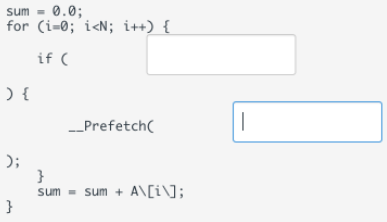
\includegraphics{assets/prefetch-code.png}
        \end{center}

        Ans: \\
        (a) \texttt{i \% 4 == 0}\\
        (b) \texttt{\&A[i + 10])}

        \item (with reference to question 4) Assume that prefetching increases instruction count by 5\%, removes L1 
        miss penalty completely, but does not change L1 miss rate (remember, prefetches still miss in the cache), L2 
        miss rate, or L2 miss penalty. Find the new AMAT, CPI, and speedup of the program using prefetching over the 
        one that didn't.

        Ans:

        new AMAT = 4.75 cycles\\
        new CPI = 1.45 cycles\\
        speedup = 1.057X

        AMAT = L1T + L1MR $\cdot$ L2T + L1MR $\cdot$ L2MR $\cdot$ L2MT\\
        = 1 + (0.10)(0) + (0.10)(0.15)(250) = 4.75

        CPI = CPI$_0$ + MemF $\cdot$ AAT = 0.5 + (0.20)(4.75) = 1.45

        CPU time = IC $\cdot$ CPI $\cdot$ CT = (100)(1.61)(1) = 161 cycles

        new CPU time = (105)(1.45)(1) = 152.25 cycles

        speedup = $\frac{161}{152.25}$ = 1.057X

        \item Given the following initial content of the branch prediction structures, when a conditional branch A 
        (\texttt{PC 0x...A}) is encountered, what is the predicted outcome? Given the actual outcome of branch A is ``taken'', 
        show the final content of the structures. Afterward, a branch B (\texttt{PC 0x...2}) is encountered; what is 
        its predicted outcome? Given its actual outcome is ``not taken'', show the final content of the structures.

        (see paper)

        \item Given the following instructions:
        
        \texttt{A: load R1, 100(R0) // R1 = MEM[R0+100]}\\
        \texttt{B: load R2, 200(R0) // R2 = MEM[R0+200]}\\
        \texttt{C: addi R2, R2, \#1 // R2 = R2 + 1}\\
        \texttt{D: bnez R1, X // if (R1 != 0) jump to X}\\
        \texttt{F: add R3, R2, \#5  // R3 = R2 + 5}\\
        ...\\
        \texttt{X: load R4, 0(R1) // R4 = MEM[R1 + 0]}

        With initial register/memory values of:

        \texttt{R0 = 0}\\
        \texttt{R1 = 100}\\
        \texttt{R2 = 200}\\
        \texttt{R3 = 300}\\
        \texttt{R4 = 400}\\
        \texttt{R5 = 500}\\
        \texttt{MEM[100] = 11}\\
        \texttt{MEM[200] = 22}

        Suppose that we have the following scenarios:

        \begin{enumerate}
            \item
            \begin{itemize}
                \item all prior instructions have retired
                \item instructions A, B, C, and D have been dispatched
                \item instructions A and B have been issued
            \end{itemize}

            \item
            \begin{itemize}
                \item instructions A, B, C, D, E, and F have been dispatched
                \item instructions B and C have completed execution without exception
                \item instruction E has been predicted as NOT TAKEN
            \end{itemize}

            \item
            \begin{itemize}
                \item instructions A and B have retired
                \item instructions D and F have completed execution without exception
                \item instruction E has completed execution and it was determined that the true branch outcome is TAKEN, 
                but E was predicted as NOT TAKEN, hence E was mispredicted (treat as exception)
            \end{itemize}

            \item show the content of the register file at the time right before and after the pipeline is 
            flushed to handle the branch misprediction at E
        \end{enumerate}

        Ans: (see paper)

    \end{enumerate}

\end{document}